\documentclass[sigconf,nonacm]{acmart}

%% Enable subfigures
\usepackage{subfigure}
%% Enable numbers in scientific format.
\usepackage{siunitx}
%% Enable enumerate start from.
\usepackage{enumitem}

%% Enable theorems
\newtheorem{theorem}{Theorem}[section]
\newtheorem{lemma}[theorem]{Lemma}

%% Enable algorithms
\usepackage{algorithm}
\usepackage[noend]{algpseudocode}
\let\ReturnInline\Return
\renewcommand{\Return}{\State\ReturnInline}
\algrenewcommand\algorithmicrequire{$\rhd$}
\algrenewcommand\algorithmicensure{$\square$}

%% Fonts used in the template cannot be substituted; margin 
%% adjustments are not allowed.
\AtBeginDocument{%
  \providecommand\BibTeX{{%
    \normalfont B\kern-0.5em{\scshape i\kern-0.25em b}\kern-0.8em\TeX}}}

%% Rights management information.
\setcopyright{acmcopyright}
\copyrightyear{2018}
\acmYear{2018}
\acmDOI{XXXXXXX.XXXXXXX}

%% These commands are for a PROCEEDINGS abstract or paper.
\acmConference[Conference acronym 'XX]{Make sure to enter the correct
  conference title from your rights confirmation emai}{June 03--05,
  2018}{Woodstock, NY}
%% Title of the proceedings is different from ``Proceedings of ...''?
% \acmBooktitle{Woodstock '18: ACM Symposium on Neural Gaze Detection,
%  June 03--05, 2018, Woodstock, NY} 
% \acmPrice{15.00}
% \acmISBN{978-1-4503-XXXX-X/18/06}

%% Submission ID.
% \acmSubmissionID{123-A56-BU3}

%% Use the "author year" style of citations and references?
% \citestyle{acmauthoryear}

%% Message
\newcommand{\kk}[1]{{{\color{red} #1}}}
\newcommand{\ds}[1]{{{\color{blue} #1}}}
\newcommand{\su}[1]{{{\color{green} #1}}}

%% Ignore block
\newcommand{\ignore}[1]{}

%% Macros
\newcommand{\Lou}{\textit{Louvain}}
\newcommand{\LPA}{\textit{LPA}}
\newcommand{\Hyb}{\textit{Hybrid Louvain-LPA}}
\newcommand{\Sta}{\textit{Static}}
\newcommand{\Nai}{P-ND}
\newcommand{\DelOrg}{\textit{$\Delta$-screening}}
\newcommand{\Del}{P-DDS}
\newcommand{\Fro}{P-DF}
\newcommand{\StaLou}{\textit{Static Louvain}}
\newcommand{\NaiLou}{$\text{P-ND}_\text{L}$}
\newcommand{\DelLou}{$\text{P-DDS}_\text{L}$}
\newcommand{\FroLou}{$\text{P-DF}_\text{L}$}
\newcommand{\StaLPA}{\textit{Static LPA}}
\newcommand{\NaiLPA}{$\text{P-ND}_\text{LPA}$}
\newcommand{\DelLPA}{$\text{P-DDS}_\text{LPA}$}
\newcommand{\FroLPA}{$\text{P-DF}_\text{LPA}$}
\newcommand{\FroHyb}{$\text{P-DF}_\text{H}$}




\begin{document}

%% Full title of the paper.
\title[GVEL: Fast Graph Loading in Edgelist and Compressed Sparse Row (CSR) formats]{GVEL: Fast Graph Loading in Edgelist and\\ Compressed Sparse Row (CSR) formats}

%% Short title to be used in page headers (optional).
% \title[short title]{full title}
% \subtitle{Something other than the title}

%% Authors and their affiliations.
\author{Subhajit Sahu}
\email{subhajit.sahu@research.iiit.ac.in}
\affiliation{%
  \institution{IIIT Hyderabad}
  \streetaddress{Professor CR Rao Rd, Gachibowli}
  \city{Hyderabad}
  \state{Telangana}
  \country{India}
  \postcode{500032}
}

%% Concise author list in page headers.
%\renewcommand{\shortauthors}{Sahu, Kothapalli, and Banerjee, et al.}

%% Show page numbers.
\settopmatter{printfolios=true}

%% Short summary of the work to be presented in the article.
\begin{abstract}
Efficient IO techniques are crucial in high-performance graph processing frameworks like Gunrock and Hornet, as fast graph loading is essential to minimize processing time and reduce system/cloud usage charges. This research study presents approaches for efficiently reading an Edgelist from a text file and converting it to a Compressed Sparse Row (CSR) representation. On a server with dual 16-core Intel Xeon Gold 6226R processors and MegaRAID SAS-3 storage, our approach, which we term as \textit{GVEL}, outperforms Hornet, Gunrock, and PIGO by significant margins in CSR reading, exhibiting an average speedup of $78\times$, $112\times$, and $1.8\times$, respectively. For Edgelist reading, GVEL is $2.6\times$ faster than PIGO on average, and achieves a Edgelist read rate of $1.9$ billion edges/s. For every doubling of threads, GVEL improves performance at an average rate of $1.9\times$ and $1.7\times$ for reading Edgelist and reading CSR respectively.
\end{abstract}

%% The code below is generated by the tool at http://dl.acm.org/ccs.cfm.
\begin{CCSXML}
<ccs2012>
<concept>
<concept_id>10003752.10003809.10003635</concept_id>
<concept_desc>Theory of computation~Graph algorithms analysis</concept_desc>
<concept_significance>500</concept_significance>
</concept>
</ccs2012>
\end{CCSXML}

% \ccsdesc[500]{Theory of computation~Graph algorithms analysis}

%% Pick words that accurately describe the work being presented.
\keywords{Memory-mapped IO, Parallel Edgelist reading, Parallel CSR reading}

% \received{20 February 2007}
% \received[revised]{12 March 2009}
% \received[accepted]{5 June 2009}



%% Process the author and title information.
\maketitle

\section{Introduction}
\label{sec:introduction}
Graphs are fundamental data structures in many applications, such as computer networks, recommendation systems, and circuit design. In recent years, a number of high performance graph processing frameworks have emerged. State-of-the-art frameworks include Gunrock \cite{wang2016gunrock}, Hornet \cite{busato2018hornet}, Ligra \cite{shun2013ligra}, and Galois \cite{nguyen2013lightweight}.\ignore{These frameworks have demonstrated efficient computation on billion-scale graphs.} Their emphasis lies in accelerating graph analytics tasks by providing high-performance kernels tailored to diverse datasets.

Unfortunately, loading graph data is a significant bottleneck in such frameworks. In fact, the cost of loading data can dominate the overall processing time --- especially as computational capabilities continue to improve\ignore{\cite{gabert2021pigo}}. Gabert and Çatalyürek \cite{gabert2021pigo} observe that\ignore{even on high-performance shared-memory graph systems running billion-scale graphs,} reading the graph from file systems, on such frameworks, takes multiple orders of magnitude longer than running the computational kernel. This slowdown not only causes a disconnect for end users and a loss of productivity for researchers\ignore{/developers}, but also increases the system/cloud usage charges. Fast loading of graphs is thus, crucial\ignore{for minimizing the time it takes to start processing and analyzing the graph data}.\ignore{This motivates us to work on efficient IO techniques. These not only improve response time, but also help lower system / cloud usage charges.}

In modern frameworks like Gunrock, loading graph data from ASCII-based file formats, specifically using the Coordinate (COO) format, is a major bottleneck. To load the graph as an Edgelist, these frameworks typically follow a sequential process of opening the input file, reading the entries one by one, and inserting them into an array. If the goal is to access the graph in the Compressed Sparse Row (CSR) format, which is often the case --- due to its storage efficiency and locality benefits, additional steps are required. These include computing the out-degrees of vertices from the Edgelist, performing prefix sum to determine the offsets of outgoing edges in the CSR representation, and then populating the CSR arrays with edges from the Edgelist. All these operations are carried out sequentially, contributing to the overall loading time.

Many graph processing frameworks\ignore{have showcased efficient computation on large-scale graphs, they}, thus, still rely on sequential I/O. This is likely due to the belief that I/O devices tend to be slow (relative to the CPU), and that achieving parallel I/O necessitates specialized systems.\ignore{Graph and matrix I/O times are seldom reported in the literature.} However, modern IO devices are fast, and implementing only sequential I/O fails to exploit the capabilities of modern Hard Disk Drives (HDDs), Redundant Array of Independent Disks (RAID) controllers, and Non-Volatile Memory (NVM) \cite{gabert2021pigo}. A number of disk-based out-of-memory graph processing systems/frameworks\ignore{\cite{zhu2015gridgraph, cheng2015venus, chi2016nxgraph, ai2017squeezing, ma2017garaph, maass2017mosaic, wu2018redio, ai2018clip, jun2018grafboost, zhang2018wonderland}} \cite{kyrola2012graphchi, han2013turbograph, roy2013x, najeebullah2014bishard, lin2014mmap, zheng2015flashgraph, wang2021scaleg} focus on loading large graphs stored in binary formats. However, a majority of graph datasets exist in serialized human-readable data exchange formats.\ignore{To address this, our focus lies on efficiently loading graphs stored in plain text formats.}

To address these challenges, Gabert and Çatalyürek introduce PIGO \cite{gabert2021pigo}, a header-only, dependency-free C++11 parallel graph loader that supports loading graphs in memory as Edgelists or CSR. PIGO leverages memory mapping, a mechanism that maps a file or part of a file into the virtual memory space\ignore{so that files on the disk can be accessed as if they were in memory} \cite{lin2014mmap}, to optimize file reading. This eliminates the need for repeated system calls, resulting in reduced context-switch overhead and improved efficiency, particularly if the kernel\ignore{accurately} predicts the accessed pages ahead of time.

However, we have identified a few issues with PIGO. Firstly, when reading entries from the input file, PIGO divides the file length equally among threads, potentially leading to slower overall performance as faster threads wait for slower ones. Secondly, PIGO utilizes a two-pass approach for loading graphs into memory as Edgelists, which involves first counting newlines to determine the number of edges and associated offsets for each thread, and then parsing and populating the Edgelist. This method is inefficient compared to a single-pass approach. When converting the Edgelist to a CSR representation, PIGO globally computes vertex degrees using atomics, uses it compute the offsets array of the global CSR, and iterates through the Edgelist to atomically populate the targets array of the global CSR. This global computation of vertex degrees, and directly operating on the shared CSR can lead to high contention between threads, especially on graphs with high average degree. Further, PIGO populates the targets array of the CSR with static load balancing, potentially leading to load imbalances among threads. Finally, when reading Matrix Market (MTX) files, a format commonly used for storing sparse graphs/matrices, PIGO disregards specified attributes, resulting in lower reported runtimes for symmetric graphs (the authors of PIGO plan to address this\ignore{in the future}).

In this technical report, we propose GVEL\footnote{\url{https://github.com/puzzlef/graph-csr-openmp}}. Similar to PIGO, it employs memory mapping and parallelization to optimize graph loading. However, GVEL improves upon PIGO by efficiently processing the graph as per-thread Edgelists in a single pass through overallocation of memory via memory mapping. Note that this does not waste memory, as untouched pages are never mapped to DRAM. To convert the per-thead Edgelists to CSR, GVEL computes four independent sets of vertex degrees (which, when summed up for each vertex, represents the global degree of each vertex), and uses it to generate the global CSR representation in a novel staged manner. It does this by first obtaining $4$ independent sets of CSRs, and then combining them together, in parallel, to form a global CSR. This minimizes the contention between threads\ignore{, which we observe to be a significant bottleneck for converting an Edgelist to CSR}. These techniques allow GVEL to achieve a $2.6\times$ speedup over PIGO for loading graphs into memory as Edgelists, and a speedup of $1.8\times$ for loading graphs into memory as CSRs (i.e., reading the graph as per-thread Edgelists and then converting it to CSR). Our techniques may also be used to convert in-memory Edgelists (an update friendly data structure), to a CSR (a space efficient and locality efficient data structure).




% x Why do HP G frameworks load graphs slowly?
% x A quick glimpse of how they do it.
% x Why do the persist with sequential IO? (Modern IO is fast)
% x What are the HP IO interfaces? (MMAP)
% x Which graphs frameworks make use of mmap? (external memory frameworks)
% x What do they focus on? (binary graph formats)
% x Why is fast loading of serialized formats important? (human readable data exchange format)
% x What have Gabert et al. done in PIGO?
% x How do we improve upon it? (link to code)

% - Measure EL, CSR, EL + CSR ...
% - Details of NVME, as much as possible.
% - Indirect comparison with Ligra, GAPbs, and Galois (PIGO).
% - Details of other graphs processing frameworks, and the above
% -- cugraph
% -- networkit
% -- igraph?
% -- gunrock
% -- hornet
% -- graphblast

% - adjust csr partitions
% - adjust csr partitions (convert csr only)
% - adjust block size
% - read EL, convert CSR split on graphs

% - Why fast graph loading is important?
% - Extremely high cost of loading compared to computation.
% - An issue with even popular graph processing frameworks.
% - Modern IO is fast (compared to CPU performance).
% - Storage capacities increasing, bandwidth is high, CPUs as not as fast as they used to be.
% - Common graph file formats (COO, MTX).
% - Common memory storage formats (Edgelist, CSR).
% - Work presented in this paper.




%% - Use --- for a dash.
%% - Use ``camera-ready'' for quotes.
%% - Use {\itshape very} or \textit{very} for italicized text.
%% - Use \verb|acmart| or {\verb|acmart|} for mono-spaced text.
%% - Use \url{https://capitalizemytitle.com/} for URLs.
%% - Use {\bfseries Do not modify this document.} for important boldface details.
%% - Use \ref{fig:name} for referencing.

%% For a block of pre-formatted text: 
% \begin{verbatim}
%   \renewcommand{\shortauthors}{McCartney, et al.}
% \end{verbatim}

%% For a list of items:
% \begin{itemize}
% \item the ``ACM Reference Format'' text on the first page.
% \item the ``rights management'' text on the first page.
% \item the conference information in the page header(s).
% \end{itemize}

%% For a table:
% \begin{table}
%   \caption{Frequency of Special Characters}
%   \label{tab:freq}
%   \begin{tabular}{ccl}
%     \toprule
%     Non-English or Math&Frequency&Comments\\
%     \midrule
%     \O & 1 in 1,000& For Swedish names\\
%     $\pi$ & 1 in 5& Common in math\\
%     \$ & 4 in 5 & Used in business\\
%     $\Psi^2_1$ & 1 in 40,000& Unexplained usage\\
%   \bottomrule
% \end{tabular}
% \end{table}

%% For a full-width table:
% \begin{table*}
%   \caption{Some Typical Commands}
%   \label{tab:commands}
%   \begin{tabular}{ccl}
%     \toprule
%     Command &A Number & Comments\\
%     \midrule
%     \texttt{{\char'134}author} & 100& Author \\
%     \texttt{{\char'134}table}& 300 & For tables\\
%     \texttt{{\char'134}table*}& 400& For wider tables\\
%     \bottomrule
%   \end{tabular}
% \end{table*}


%% For inline math:
% \begin{math}
%   \lim_{n\rightarrow \infty}x=0
% \end{math},

%% For a numbered equation:
% \begin{equation}
%   \lim_{n\rightarrow \infty}x=0
% \end{equation}

%% For an unnumbered equation:
% \begin{displaymath}
%   \sum_{i=0}^{\infty} x + 1
% \end{displaymath}

%% For a figure:
% \begin{figure}[h]
%   \centering
%   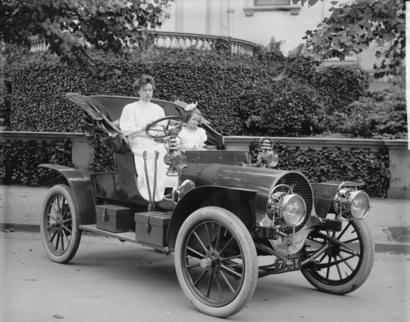
\includegraphics[width=\linewidth]{inc/sample-franklin}
%   \caption{1907 Franklin Model D roadster. Photograph by Harris \&
%     Ewing, Inc. [Public domain], via Wikimedia
%     Commons. (\url{https://goo.gl/VLCRBB}).}
%   \Description{A woman and a girl in white dresses sit in an open car.}
% \end{figure}

%% For a teaser figure.
% \begin{teaserfigure}
%   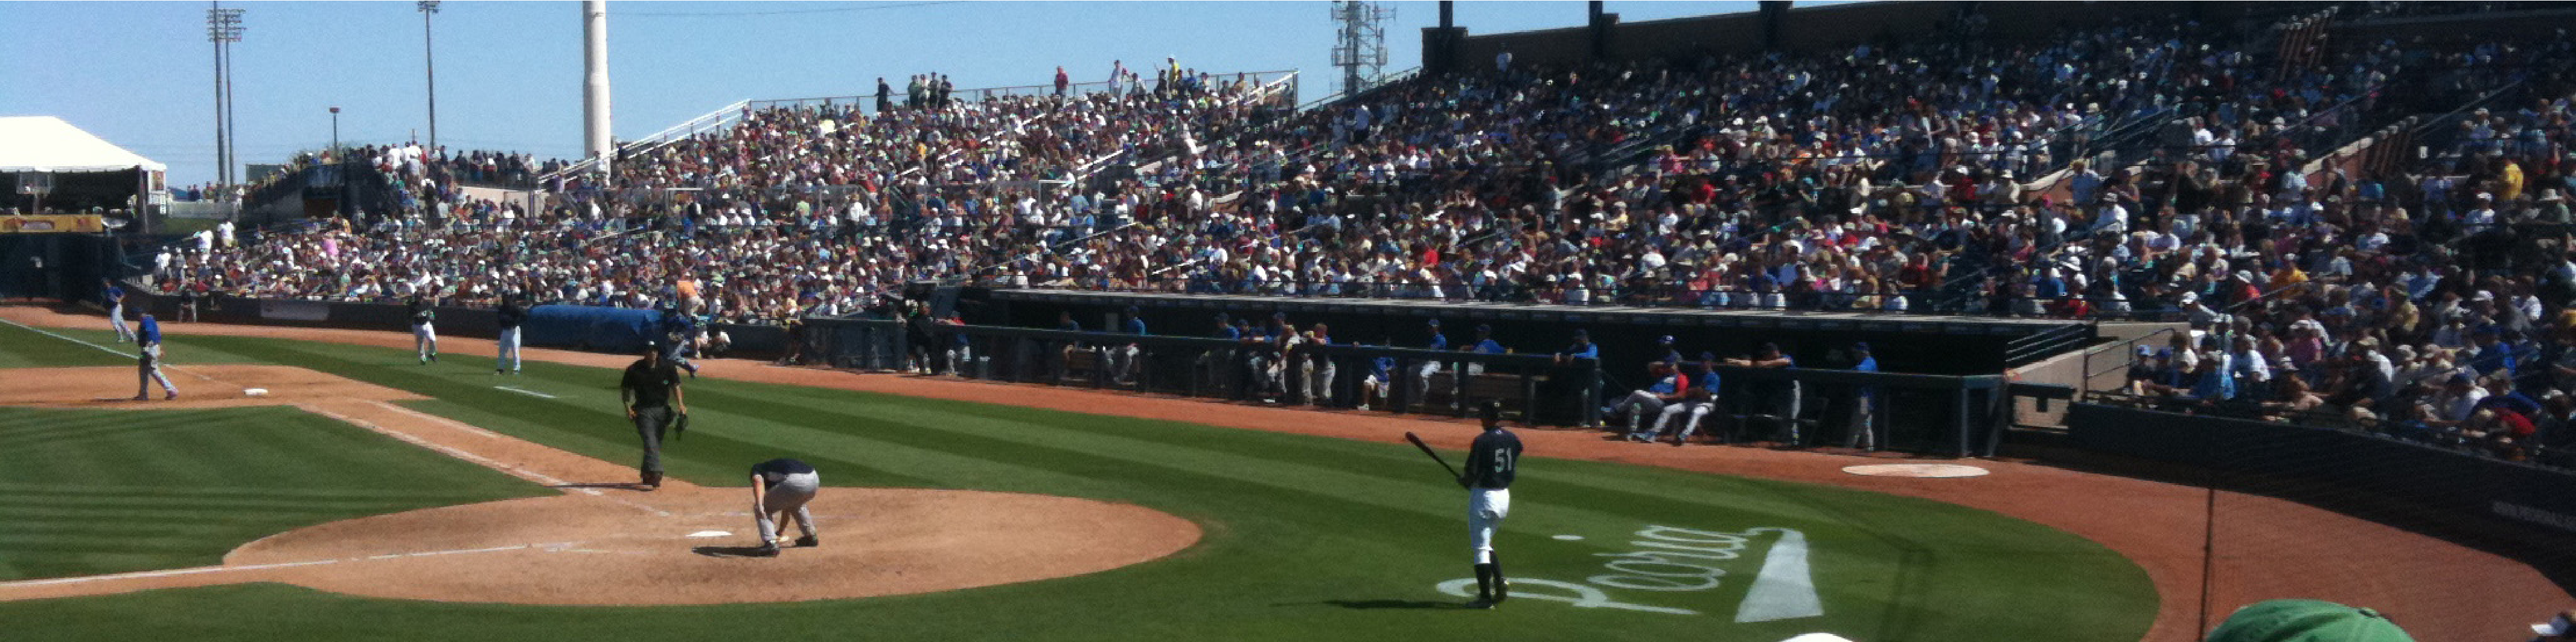
\includegraphics[width=\textwidth]{sampleteaser}
%   \caption{figure caption}
%   \Description{figure description}
% \end{teaserfigure}


\section{Related work}
\label{sec:related}
Lin et al. \cite{lin2014mmap} use the fundamental memory mapping capability of all modern hardware to create fast and scalable graph algorithms. They are able to to process 6.6 billion edge Yahoo web graph faster than other graph processing frameworks, such as TorboGraph and GraphChi, with reduced complexity - both in terms of simpler data structures, and fewer lines of code. They benefit from existing page replacement policies, such as LRU.

Song et al. \cite{song2016efficient} optimize Linux's memory mapped IO (mmio) for fast storage devices. Their results indicate that mmap can be used effectively with fast storage.

Malliotakis et al. \cite{malliotakis2021hugemap} present HugeMap, a custom mmio path in the Linux kernel that uses huge pages for file-backed mappings to accelerate applications with sequential I/O access patterns or large I/O operations. Their experiments show up to higher throughput and lower system time, compared to regular page configurations.

Papagiannis et al. \cite{papagiannis2020optimizing} propose FastMap, an alternative design for the memory-mapped I/O path in Linux that provides scalable access to fast storage devices in multi-core servers, by reducing synchronization overhead in the common path. FastMap also increases device queue depth, an important factor to achieve peak device throughput. Our experimental analysis shows that FastMap scales up to 80 cores and provides up to 11.8× more IOPS compared to mmap using null\_blk. Additionally, it provides up to 5.27x higher throughput using an Optane SSD. We also show that FastMap is able to saturate state-of-the-art fast storage devices when used by a large number of cores, where Linux mmap fails to scale.

Essen et al. \cite{van2015di} present DI-MMAP, a high-performance runtime that memory-maps large external data sets into an application’s address space and shows better performance than the Linux mmap system call.

Wang et al. \cite{wang2019lgraph} present LGraph, a unified data model and API for productive open-source hardware design. Key features of LGraph include a
unified data model and API, a fast memory mapped library design, integration with third-party tools and hierarchical design traversal for third-party tools.

Papagiannis et al. \cite{papagiannis2021memory} present Aquila, a library OS that allows applications to reduce I/O overhead by customizing the memory-mapped I/O (mmio) path for files or storage devices. Compared to Linux mmap, Aquila (a) offers full mmio compatibility and protection to minimize application modifications, (b) allows applications to customize the DRAM I/O cache, its policies, and access to storage devices, and (c) significantly reduces I/O overhead. Aquila achieves its mmio compatibility, flexibility, and performance by placing the application in a privileged domain, non-root ring 0. We show the benefits of Aquila in two cases: (a) Using mmio in key-value stores to reduce I/O overhead and (b) utilizing mmio in graph processing applications to extend the memory heap over fast storage devices. Aquila requires 2.58× fewer CPU cycles for cache management in RocksDB, compared to user-space caching and read/write system calls and results in 40\% improvement in request throughput. Finally, we use Ligra, a graph processing framework, to show the efficiency of Aquila in extending the memory heap over fast storage devices. In this case, Aquila results in up to 4.14× lower execution time compared to Linux mmap.

Alverti et al. \cite{alverti2022daxvm} propose DaxVM, a design that extends the OS virtual memory and file system layers leveraging persistent memory attributes to provide a fast and scalable DAX-mmap interface. DaxVM eliminates paging costs through pre-populated file page tables, supports faster and scalable virtual address space management for ephemeral mappings, performs unmappings asynchronously, bypasses kernel-space dirty-page tracking support, and adopts asynchronous block pre-zeroing. We implement DaxVM in Linux and the ext4 file system targeting xS6-64 architecture. DaxVM mmap achieves 4.9x higher throughput than default mmap for the Apache webserver and up to 1.5x better performance than read system calls. It provides similar benefits for text search. It also provides fast boot times and up to 2.95x better throughput than default mmap for PMem-optimized key-value stores running on a fragmented ext4 image. Despite designed for direct access to byte-addressable storage, various aspects of DaxVM are relevant for efficient access to other high performant storage mediums.

Song et al. \cite{song2012low} examine linux virtual memory subsystem and mmap() I/O path to figure out the influence of low-latency storage devices on the existing virtual memory subsystem. Also, we suggest some optimization policies to reduce the overheads of mmap() I/O and implement the prototype in a recent Linux kernel. Our solution guarantees that 1) memory-mapped I/O will be several times faster than read-write I/O when cache-hit ratio becomes high, and 2) the former will show at least the performance of the latter even when cache-miss frequently occurs and the overhead of mapping/unmapping pages becomes significant, which are not achievable by the existing virtual memory subsystem.

Imamura and Yoshida \cite{imamura2019poster} propose AR-MMAP that is an asynchronous read method to reduce the write latency of applications applying memory-mapped files. It hides the read latency of block devices by reading the corresponding pages from block devices in background. As AR-MMAP requires the assistance of applications to guarantee data consistency, we modify an in-memory key-value store as a use case. We implement AR-MMAP in a Linux kernel and evaluate its performance on a server containing two types of SSDs. The evaluation results demonstrate that it reduces the execution time compared to a default kernel.

Li et al. \cite{li2019userland} propose CO-PAGER, which is a lightweight userspace memory service. CO-PAGER consists of a minimal kernel module and a userspace component. The userspace component handles (redirected) page faults, performs memory management and I/O operations and accesses NVM storage directly. The kernel module is used to update memory mapping between user and kernel space. In this way CO-PAGER can bypass the deep kernel I/O stacks and provide a flexible/customizable and efficient memory paging service in userspace. We provide a general programming interface to use the CO-PAGER service. In our experiments, we also demonstrate how the CO-PAGER approach can be applied to a MapReduce framework and improves performance for data-intensive applications.

Feng et al. \cite{feng2023tricache} propose TriCache, a cache mechanism that enables in-memory programs to efficiently process out-of-core datasets without requiring any code rewrite. It provides a virtual memory interface on top of the conventional block interface to simultaneously achieve user transparency and sufficient out-of-core performance. A multi-level block cache design is proposed to address the challenge of per-access address translations required by a memory interface. It can exploit spatial and temporal localities in memory or storage accesses to render storage-to-memory address translation and page-level concurrency control adequately efficient for the virtual memory interface.

Leis et al. \cite{leis2023virtual} propose vmcache, a buffer manager design that instead uses hardware-supported virtual memory to translate page identifiers to virtual memory addresses. In contrast to existing mmap-based approaches, the DBMS retains control over page faulting and eviction. Our design is portable across modern operating systems, supports arbitrary graph data, enables variable-sized pages, and is easy to implement. One downside of relying on virtual memory is that with fast storage devices the existing operating system primitives for manipulating the page table can become a performance bottleneck. As a second contribution, we therefore propose exmap, which implements scalable page table manipulation on Linux. Together, vmcache and exmap provide flexible, efficient, and scalable buffer management on multi-core CPUs and fast storage devices.






Graph processing frameworks
PIGO


\section{Preliminaries}
\label{sec:preliminaries}
\subsection{PageRank}
\label{sec:PageRank}

Consider a directed graph $G(V, E, w)$, with $V$ ($n = |V|$) as the set of vertices and $E$ ($m = |E|$) as the set of edges. The PageRank $R[v]$ of a vertex $v \in V$ in this graph measures its importance based on incoming links and their significance. Equation \ref{eq:pr} defines the PageRank calculation for a vertex $v$ in $G$. $G.in(v)$ and $G.out(v)$ represent incoming and outgoing neighbors of $v$, and $\alpha$ is the damping factor (usually $0.85$). Initially, each vertex has a PageRank of $1/n$, and the \textit{power-iteration} method updates these values iteratively until they converge within a specified tolerance $\tau$, indicating that convergence has been achieved.

% \begin{equation}
% \label{eq:pr}
%     R[v] = \alpha \times \sum_{u \in G.in(v)} \frac{R[u]}{|G.out(u)|} + \frac{1 - \alpha}{n}
% \end{equation}




\subsection{Gini coefficient}

Gini coefficient $G$ is a value which represents income/wealth inequality within a nation or group. It ranges from $0$ to $1$, with $0$ representing total equality and $1$ representing total inequality. It is calculated from the Lorenz curve, which plots cumulative income/wealth against cumulative number of households/people. It is calculated using Equation \ref{eq:gini}, where $A$ is the area between the line of perfect equality and the Lorenz curve, and $B$ is the total area under the line of perfect equality.

% \begin{equation}
% \label{eq:gini}
%   G = \frac{A}{A+B}
% \end{equation}

\begin{table}[!ht]
  \centering
  \caption{In our experiments, we use a list of 17 graphs. Each graph has its edges duplicated in the reverse direction to make them undirected, and a weight of 1 is assigned to each edge. The table lists the total number of vertices ($|V|$), total number of edges ($|E|$) after making the graph undirected, and the file size ($F_{size}$) for each graph. The number of vertices and edges are rounded to the nearest thousand or million, as appropriate.}
  \label{tab:dataset}
  \begin{tabular}{|c||c|c|c|}
    \toprule
    \textbf{Graph} &
    \textbf{\textbf{$|V|$}} &
    \textbf{\textbf{$|E|$}} &
    \textbf{\textbf{$F_{size}$}} \\
    \midrule
    \multicolumn{4}{|c|}{\textbf{Web Graphs (LAW)}} \\ \hline
    indochina-2004$^*$ & 7.41M & 341M & 2.9 GB \\ \hline
    arabic-2005$^*$ & 22.7M & 1.21B & 11 GB \\ \hline
    uk-2005$^*$ & 39.5M & 1.73B & 16 GB \\ \hline
    webbase-2001$^*$ & 118M & 1.89B & 18 GB \\ \hline
    it-2004$^*$ & 41.3M & 2.19B & 19 GB \\ \hline
    sk-2005$^*$ & 50.6M & 3.80B & 33 GB \\ \hline
    \multicolumn{4}{|c|}{\textbf{Social Networks (SNAP)}} \\ \hline
    com-LiveJournal & 4.00M & 69.4M & 480 MB \\ \hline
    com-Orkut & 3.07M & 234M & 1.7 GB \\ \hline
    \multicolumn{4}{|c|}{\textbf{Road Networks (DIMACS10)}} \\ \hline
    asia\_osm & 12.0M & 25.4M & 200 MB \\ \hline
    europe\_osm & 50.9M & 108M & 910 MB \\ \hline
    \multicolumn{4}{|c|}{\textbf{Protein k-mer Graphs (GenBank)}} \\ \hline
    kmer\_A2a & 171M & 361M & 3.2 GB \\ \hline
    kmer\_V1r & 214M & 465M & 4.2 GB \\ \hline
  \bottomrule
  \end{tabular}
  \end{table}



\section{Approach}
\label{sec:approach}
\subsection{Reading Edgelist from text file}

We attempt a number of approaches to read Edgelist from text file into in-memory Edgelist(s), given in Sections \ref{sec:el-fstream-plain}-\ref{sec:el-mmap-custom}. Among these, we find using \texttt{mmap()} with custom number parsers (\textit{mmap-custom}) to be the best approach. The pseudocode for \textit{mmap-custom} is given Algorithm \ref{alg:el}.


\subsubsection{\texttt{ifstream} with \texttt{getline()} and \texttt{>>} operator (\textit{fstream-plain})}
\label{sec:el-fstream-plain}

In this approach, we utilize C++'s \texttt{ifstream} to open the file, and read the edges line by line with \texttt{getline()}. If the graph is unweighted, we read the source and target vertex ids as 64-bit unsigned integers, using \texttt{>>} operator, into pre-allocated source and target arrays based on information in the file header. If the graph is weighted, we also read the weights as 32-bit floating-point numbers into another pre-allocated array. This process is sequential, given that streams are inherently sequential.


\subsubsection{\texttt{ifstream} with \texttt{getline()} and \texttt{strto*()} (\textit{fstream-strto*})}
\label{sec:el-fstream-stro*}

In this approach, we again use \texttt{ifstream} but employ string-to-number conversion methods \texttt{strtoull()} and \texttt{strtod()} for parallel number parsing. We sequentially read a block of $L$ lines from the file, using \texttt{getline()}, and then parse each line in parallel using multiple threads. We observe that using OpenMP's dynamic scheduling, with a chunk size of $1024$, and reading a block of $L=128K$ lines to be processed in parallel offers the best performance. Parsed edges (source, target vertex ids, and edge weights) are stored separately in per-thread edge lists to avoid contention issues within a shared data structure. With 64 threads, this approach demonstrates a speedup of $8.7\times$ compared to \textit{fstream-plain}, as shown in Figure \ref{fig:optimize-el}.

\begin{figure}[hbtp]
  \centering
  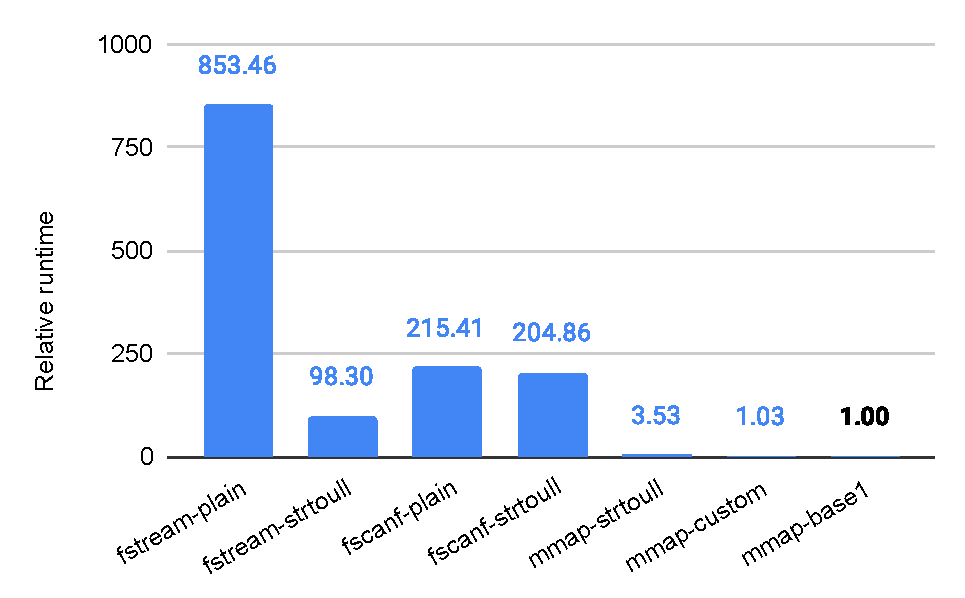
\includegraphics[width=0.99\linewidth]{out/optimize-el.pdf} \\[-2ex]
  \caption{Gini coefficient of PageRank values on 24 different graphs, comparing between PageRank values obtained with three different dead-end handling strategies: \textit{teleport from dead-ends} (\textbf{default}), \textit{self-loop dead-ends} (\textbf{loop}), and \textit{self-loop all vertices} (\textbf{loopall}).}
  \label{fig:optimize-el}
\end{figure}



\subsubsection{\texttt{fopen()} with \texttt{fgets()} and \texttt{sscanf()} (\textit{fopen-plain})}
\label{sec:el-fopen-plain}

This approach is similar to the one mentioned above (\textit{fscanf-strto*}), but we use \texttt{fgets()} on a file handle to read lines instead of \texttt{getline()}, and employ \texttt{sscanf()} to parse the edges. With 64 threads, it provided a speedup of $4.0\times$ compared to \textit{fstream-plain}.


\subsubsection{\texttt{fopen()} with \texttt{fgets()} and \texttt{strto*()} (\textit{fopen-strto*})}
\label{sec:el-fopen-strto*}

Similar to the previous approach (\textit{fopen-plain}), this one uses \texttt{fgets()} to read lines from the text file, but replaces \texttt{sscanf()} with \texttt{strtoull()} and \texttt{strtod()}. This proves faster due to the absence of a format string. At 64 threads, its speedup is $1.1\times$ over \textit{fopen-plain}.


\subsubsection{\texttt{mmap()} with \texttt{strto*()} (\textit{mmap-strto*})}
\label{sec:el-mmap-strto*}

In this approach, we map the file to memory with \texttt{mmap()}, and process the edges in parallel by partitioning the file into blocks of $C$ characters. Each block is dynamically assigned (using OpenMP's dynamic schedule) to a free thread. If the assigned block contains partial lines at either end, the thread repositions it, by shifting to the right to eliminate partial lines. This involves skipping the partial line at the beginning and including the partial line from the end. We observe that issuing \texttt{madvice(MADV\_WILLNEED)}, and using a block size of $\beta=256K$ characters offers the best performance. To parse the source/target vertex ids and edge weights, we use \texttt{strtoull()} and \texttt{strtod()}. Each thread stores the parsed edges in per-thread Edgelists. With 64 threads, it provides a speedup of $58.5\times$ over \textit{fopen-strto*}, as show in Figure \ref{fig:optimize-el}.


\subsubsection{\texttt{mmap()} with custom number parsers (\textit{mmap-custom})}
\label{sec:el-mmap-custom}

This is similar to the approach mentioned above (\textit{mmap-strto*}), but we use our own functions for parsing whole numbers and floating-point numbers. In addition, as vertex ids start with $1$, we decrement $1$ from the vertex ids after parsing it and before appending them to per-thread Edgelists. Surprisingly, this leads to $40-50\%$ drop in performance. Converting the $weighted$ flag (see Algorithm \ref{alg:el}) to a template parameter solves this issue. This indicates that the issue was related to the loop code not being able to fit in the code cache of the processor and using a template allowed it to fit in the cache. Accordingly, we also recommend using $symmetric$ flag as a template parameter instead. With 64 threads, it provides a speedup of $3.5\times$ over \textit{mmap-strto*}. We also attempted to use custom SIMD instructions to parse numbers, along with \texttt{vzeroupper} instruction to clear SSE/AVX registers, but it did not provide additional performance improvement.

\begin{figure}[hbtp]
  \centering
  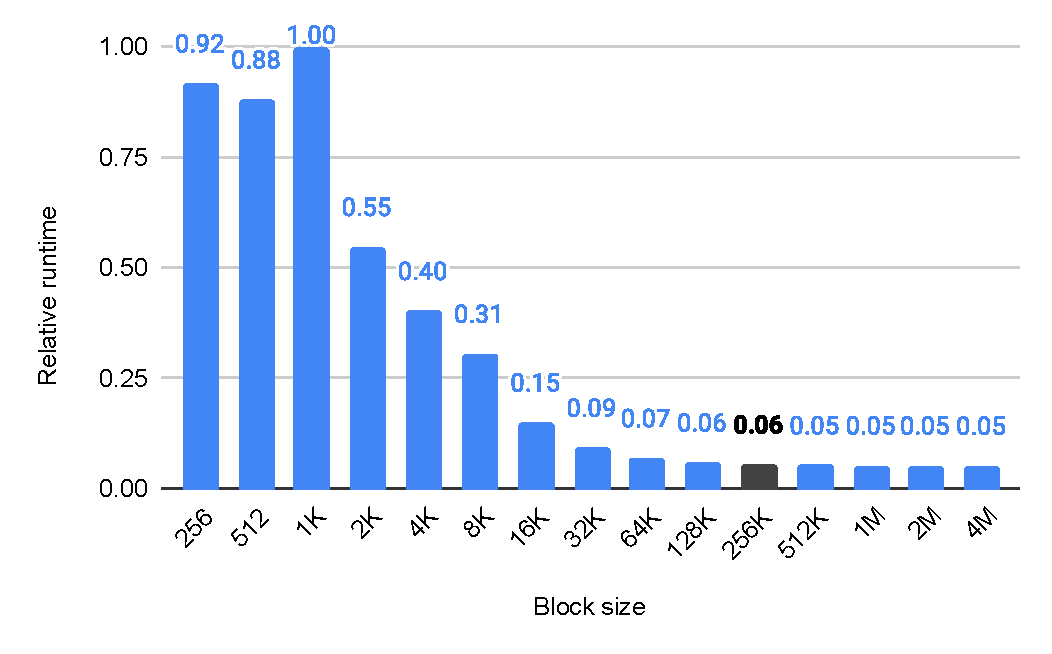
\includegraphics[width=0.99\linewidth]{out/adjust-blocksize.pdf} \\[-2ex]
  \caption{Relative runtime of reading per-thread Edgelists with varying block sizes (each thread is dynamically assigned a block of characters to process), from $256$ bytes to $4M$ bytes, using \texttt{mmap} with custom integer/float parsing functions along with making vertex id 0-based (\textit{mmap-custom}).}
  \label{fig:adjust-blocksize}
\end{figure}

\begin{figure}[hbtp]
  \centering
  \subfigure[Relative runtime for converting Edgelists to CSR]{
    \label{fig:adjust-csrpartitions--convert}
    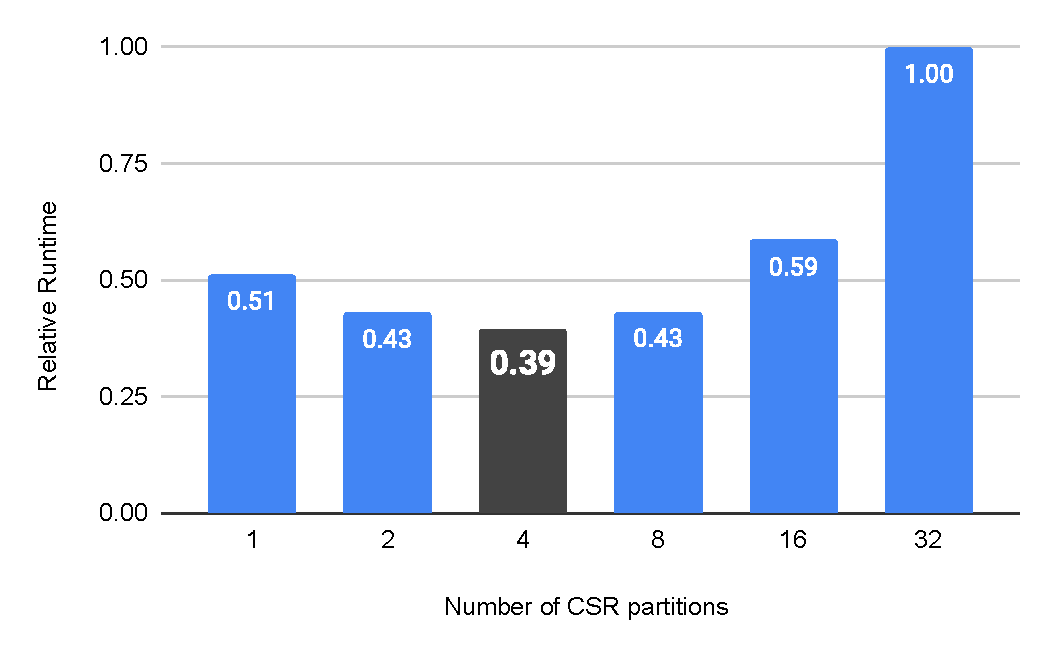
\includegraphics[width=0.98\linewidth]{out/adjust-csrpartitions-convert.pdf}
  }
  \subfigure[Relative runtime for reading graph as Edgelists, and converting to CSR]{
    \label{fig:adjust-csrpartitions--full}
    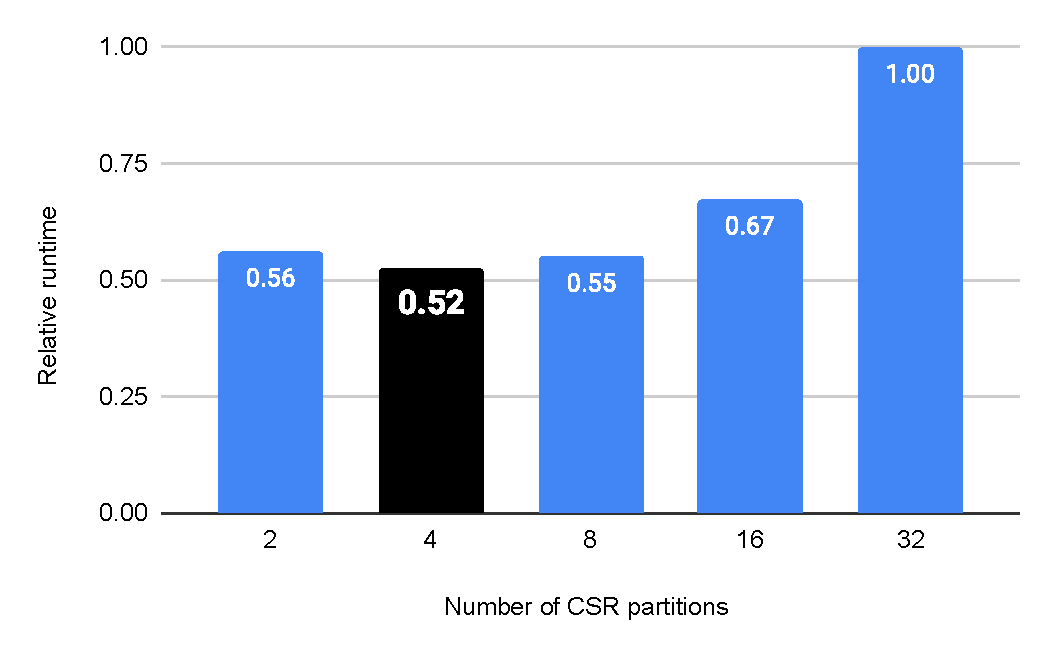
\includegraphics[width=0.98\linewidth]{out/adjust-csrpartitions-full.pdf}
  } \\[-2ex]
  \caption{Relative runtime of reading per-thread Edgelists, obtaining $p$-partition degrees, converting to $p$-partition CSR, and combini to global CSR, with the number of partitions $p$ varying from $1$ to $32$. Here, $p > 1$ implies a multi-stage approach for generating CSR, which minimizes contention\ignore{between threads}.}
  \label{fig:adjust-csrpartitions}
\end{figure}

\begin{algorithm}[hbtp]
\caption{Reading Edge-list from file.}
\label{alg:el}
\begin{algorithmic}[1]
\Require{$pdegrees$: Per partition vertex degrees (output)}
\Require{$edges$: Per thread sources, targets, and weights of edges (output)}
\Require{$data$: Memory mapped file data}
\Ensure{$counts$: Number of edges read per thread (output)}
\Ensure{$symmetric$: Is graph symmetric?}
\Ensure{$weighted$: Is graph weighted?}
\Ensure{$\beta$: Size of each block that is processed per thread}
\Ensure{$\rho$: Number of partitions for counting vertex degrees}
\Ensure{$t$: Current thread}

\Statex

\Function{getBlock}{$data, i$} \label{alg:frontier--main-begin}
  \State $[d, D] \gets data$
  \State $b \gets d+i$ \textbf{;} $B \gets min(b+\beta, D)$
  \If{$b \neq d$ \textbf{and not} $isNewline(b-1)$}
    \State $b \gets findNextLine(b, D)$
  \EndIf
  \If{$B \neq d$ \textbf{and not} $isNewline(B-1)$}
    \State $B \gets findNextLine(B, D)$
  \EndIf
  \Return{$[b, B]$}
\EndFunction

\Statex
  
\Function{readEdgelist}{$pdegrees, edges, data$}
  \State $counts \gets \{0\}$
  \State $[sources, targets, weights] \gets edges$
  \State $\rhd$ Load edges from text file in blocks of size $\beta$
  \ForAll{$i \in [0, \beta, 2\beta, ... |data|]$ \textbf{in parallel}}
    \State $j \gets counts[t]$
    \State $[b, B] \gets getBlock(data, i)$
    \While{$true$}
      \State $\rhd$ Read an edge from the block
      \State $u \gets v \gets 0$ \textbf{;} $w \gets 1$
      \State $b \gets findNextDigit(b, B)$
      \If{$b = B$} \textbf{break}
      \EndIf
      \State $b \gets parseWholeNumber(u, b, B)$
      \State $b \gets findNextDigit(b, B)$
      \State $b \gets parseWholeNumber(v, b, B)$
      \If{$weighted$}
        \State $b \gets findNextDigit(b, B)$
        \State $b \gets parseFloat(w, b, B)$
      \EndIf
      \State $\rhd$ Make it zero-based
      \State $u \gets u - 1$ \textbf{;} $v \gets v - 1$
      \State $\rhd$ Add the parsed edge to edgelist
      \State $sources[t][j] \gets u$
      \State $targets[t][j] \gets v$
      \If{$weighted$} $weights[t][j] \gets w$
      \EndIf
      \State $atomicAdd(pdegrees[t \bmod \rho][u], 1)$
      \State $j \gets j + 1$
      \State $\rhd$ If graph is symmetric, add the reverse edge
      \If{$symmetric$}
        \State $sources[t][j] \gets v$
        \State $targets[t][j] \gets u$
        \If{$weighted$} $weights[t][j] \gets w$
        \EndIf
        \State $atomicAdd(pdegrees[t \bmod \rho][v], 1)$
        \State $j \gets j + 1$
      \EndIf
    \EndWhile
    \State $counts[t] \gets j$
  \EndFor
  \Return{$counts$}
\EndFunction
\end{algorithmic}
\end{algorithm}

\begin{algorithm}[hbtp]
\caption{Convert Edge-list to CSR.}
\label{alg:csr}
\begin{algorithmic}[1]
\Require{$csr$: Global CSR (output)}
\Require{$pcsr$: Per partition CSR (scratch)}
\Require{$pdegrees$: Per partition vertex degrees (scratch)}
\Require{$edges$: Per thread sources, targets, and weights of edges}
\Require{$counts$: Number of edges read per thread}
\Ensure{$symmetric$: Is graph symmetric?}
\Ensure{$weighted$: Is graph weighted?}
\Ensure{$\rho$: Number of partitions for counting vertex degrees}
\Ensure{$t$: Current thread}

\Statex

\Function{convertToCsr}{$csr, pcsr, pdegrees, edges, counts$}
  \State $[offsets, edgeKeys, edgeValues] \gets csr$ \label{alg:csr--initialize-begin}
  \State $[poffsets, pedgeKeys, pedgeValues] \gets pcsr$
  \State $[sources, targets, weights] \gets edges$ \label{alg:csr--initialize-end}
  \State $\rhd$ Compute offsets
  \ForAll{$p \in [0, \rho)$} \label{alg:csr--poffsets-begin}
    \State $exclusiveScan(poffsets[p], pdegrees[p], |V|+1)$
  \EndFor \label{alg:csr--poffsets-end}
  \State $\rhd$ Populate per-partition CSR
  \ForAll{\textbf{threads in parallel}} \label{alg:csr--pcsr-begin}
    \ForAll{$i \in [0, counts[t])$}
      \State $u \gets sources[t][i]$
      \State $v \gets targets[t][i]$
      \State $j \gets atomicAdd(poffsets[t \bmod \rho][u], 1)$
      \State $pedgeKeys[t \bmod \rho][j] \gets v$
      \If{$weighted$}
        \State $pedgeValues[t \bmod \rho][j] \gets weights[t][i]$
      \EndIf
    \EndFor
  \EndFor \label{alg:csr--pcsr-end}
  \State $\rhd$ Fix per-partition offsets
  \ForAll{\textbf{threads in parallel}} \label{alg:csr--poffsets-fix-begin}
    \If{$t < \rho$}
      \State $memcpy(poffsets[t]+1, poffsets[t], |V|)$
      \State $poffsets[t][0] \gets 0$
    \EndIf
  \EndFor \label{alg:csr--poffsets-fix-end}
  \State $\rhd$ Combine per-partition degrees
  \ForAll{$u \in [0, |V|)$ \textbf{in parallel}} \label{alg:csr--poffsets-combine-begin}
    \ForAll{$p \in [1, \rho)$}
      \State $pdegrees[0][u] +\gets pdegrees[p][u]$
    \EndFor
  \EndFor \label{alg:csr--poffsets-combine-end}
  \State $\rhd$ Compute global offsets
  \State $exclusiveScan(offsets, pdegrees[0], |V|+1)$ \label{alg:csr--offsets-compute}
  \State $\rhd$ Combine per-partition CSR into one CSR
  \ForAll{$u \in [0, |V|)$ \textbf{in parallel}} \label{alg:csr--pcsr-combine-begin}
    \State $j \gets offsets[u]$
    \ForAll{$p \in [0, \rho)$}
      \State $i \gets poffsets[t][u]$
      \State $I \gets poffsets[t][u+1]$
      \ForAll{$i \in [i, I)$}
        \State $edgeKeys[j] \gets pedgeKeys[t][i]$
        \If{$weighted$}
          \State $edgeValues[j] \gets pedgeValues[t][i]$
        \EndIf
        \State $j \gets j + 1$
      \EndFor
    \EndFor
  \EndFor \label{alg:csr--pcsr-combine-end}
\EndFunction
\end{algorithmic}
\end{algorithm}


The psuedocode of the \textit{mmap-custom} approach is given in Algorithm \ref{alg:el}. It loads per-thread Edgelists from a file with the best performance, and is enacpsulated in the \texttt{readEdgelist()} function\ignore{(lines \ref{alg:el--read-edgelist-begin}-\ref{alg:el--read-edgelist-end})}. First, the counts of edges read per thread ($counts$) are initialized, and the components of per-thread Edgelists are obtained ($edges$) in lines \ref{alg:el--initialize-begin}-\ref{alg:el--initialize-end}. This is followed by a loop (lines \ref{alg:el--blocks-begin}-\ref{alg:el--blocks-end}), where each iteration processes a block of characters (of size $\beta = 256K$) in the text file in parallel across different threads. The text file is assumed to have been memory mapped as $data$. Inside the loop, $j$ keeps track of the number of edges processed by the current thread. In line \ref{alg:el--get-block}, the \texttt{getBlock()} function is called to retrieve the begin and end of current block of text ($[b, B]$), which is processed in the main loop (lines \ref{alg:el--block-begin}-\ref{alg:el--block-begin}). The main loop parses edges (lines \ref{alg:el--parse-edge-begin}-\ref{alg:el--parse-edge-end}), adjusts vertex indices to be zero-based (line \ref{alg:el--base1}), and adds them to the Edgelist of the current thread while updating per-partition vertex degrees with atomic operations (lines \ref{alg:el--add-edge-begin}-\ref{alg:el--add-edge-end}). Reverse edges are added for symmetric graphs (lines \ref{alg:el--reverse-edge-begin}-\ref{alg:el--reverse-edge-end}). Finally, counts of processed edges per thread are recorded (line \ref{alg:el--update-counts}) and returned (line \ref{alg:el--return-counts}).

The \texttt{getBlock()} function\ignore{(lines \ref{alg:el--get-block-begin}-\ref{alg:el--get-block-begin})} retrieves a block of characters to process\ignore{from the memory-mapped file}, starting from index $i$. It ensures that the block starts and ends on newline characters for proper parsing. The block size is determined by the parameter $\beta$, which is set to $256K$.




\subsection{Converting Edgelist to CSR}

Now that we have obtained per-thread Edgelists, we must now convert the Edgelists to CSR. We attempt a few of approaches for this in steps, given in Sections \ref{sec:csr-degree-global}-\ref{sec:csr-csr-partition4}. Among these, we find that obtaining CSR from vertex degrees, where the vertex degrees are computed in four separate partitions using $\bmod$ operator with the current thread id, performs the best. The pseudocode for \textit{csr-partition4} is given in Algorithm \ref{alg:csr}.


\subsubsection{Obtain global vertex degrees along with reading Edgelist (\textit{degree-global})}
\label{sec:csr-degree-global}

To convert the Edgelists to CSR, we first need to know the degree of each vertex. In this approach, we use a simple solution for this, i.e.,  we update the degree of each vertex in a single shared array using atomic operations, while reading Edgelists on each thread. The relative runtime of this approach with respect to simply reading per-thread Edgelists is $1.9\times$, as shown in Figure \ref{fig:optimize-csr}. We however observe that this results in high contention and impacts performance.

\begin{figure}[hbtp]
  \centering
  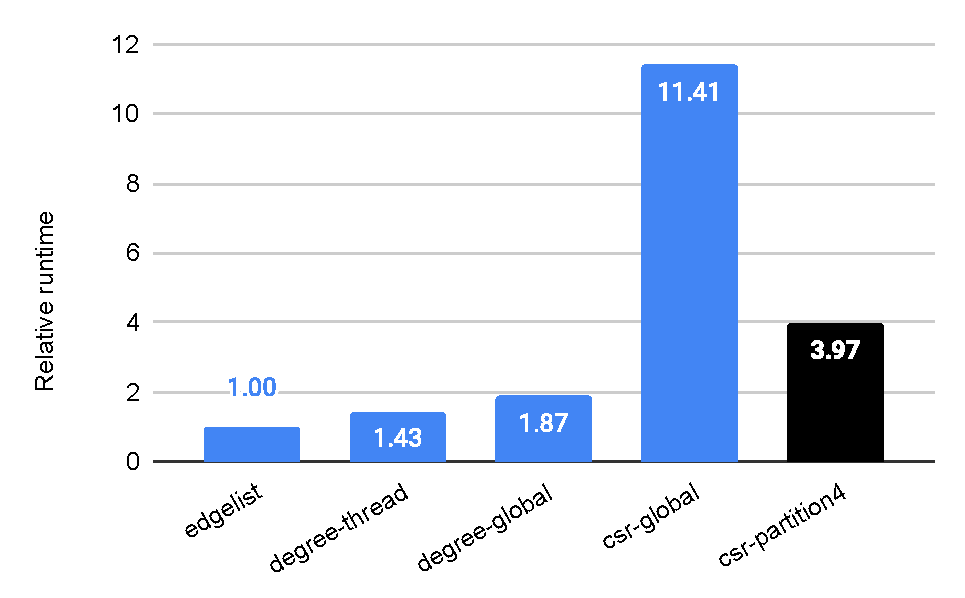
\includegraphics[width=0.99\linewidth]{out/optimize-csr.pdf} \\[-2ex]
  \caption{Gini coefficient of PageRank values on 24 different graphs, comparing between PageRank values obtained with three different dead-end handling strategies: \textit{teleport from dead-ends} (\textbf{default}), \textit{self-loop dead-ends} (\textbf{loop}), and \textit{self-loop all vertices} (\textbf{loopall}).}
  \label{fig:optimize-csr}
\end{figure}



\subsubsection{Obtain per-thread vertex degrees along with reading Edgelist (\textit{degree-thread})}
\label{sec:csr-degree-thread}

In this approach, we compute per-thread vertex degrees instead of global degrees. While this improves performance by $24\%$ compared to obtaining global vertex degrees, it requires significant additional space, and needs to be combined later to obtain global degrees. We observe that computing degrees in partitions of $4$ (using $\bmod 4$) and then combining them into a global degrees array gives us the best performance.


\subsubsection{Obtain CSR from global vertex degrees (\textit{csr-global})}
\label{sec:csr-csr-global}

Now that we have the degrees, we need to combine the per-thread Edgelists into a CSR data structure. In this approach, we first obtain global vertex degrees along with reading per-thread Edgelists (as with \textit{degree-global}), and then convert the per-thread Edgelists to a global CSR in parallel using atomic operations. As shown in Figure \ref{fig:optimize-csr}, this approach has poor performance (it is $11.4\times$ slower than simply reading Edgelists).


\subsubsection{Obtain CSR from 4-partitioned vertex degrees (\textit{csr-partition4})}
\label{sec:csr-csr-partition4}

Finally, we explore computing CSR in $k$ separate partitions and later combining them into a single global CSR. The vertex degrees are also obtained in $k$ partitions while reading Edgelist, which is then used for generating partitioned CSR. We adjust the value of $k$ from $1$ to $16$. Our observations indicate that using $4$ partitions to generate CSR and then combining them has the best performance - it offers $2.9\times$ speedup over \textit{csr-global}.

The psuedocode of the \textit{csr-partition4} approach is given in Algorithm \ref{alg:csr}. It transforms an Edgelist representation of a graph into CSR format. First, the components of global CSR ($csr$), per-partition CSRs ($pcsr$), and per-thread Edgelists ($edges$) are obtained in lines \ref{alg:csr--initialize-begin}-\ref{alg:csr--initialize-end}. The algorithm then computes offsets for each partition in parallel (lines \ref{alg:csr--poffsets-begin}-\ref{alg:csr--poffsets-begin}) using exclusive scan operations, and updates the per-partition CSRs concurrently (lines \ref{alg:csr--pcsr-begin}-\ref{alg:csr--pcsr-end}). Atomic operations ensure thread safety when updating the matrices. In lines \ref{alg:csr--poffsets-fix-begin}-\ref{alg:csr--poffsets-fix-end}, per-partition offsets are fixed as they were updated during the edge insertion process above. The algorithm then combines per-partition degrees (lines \ref{alg:csr--poffsets-combine-begin}-\ref{alg:csr--poffsets-combine-end}), computes global offsets (line \ref{alg:csr--offsets-compute}), and merges the per-partition CSRs into the global CSR (lines \ref{alg:csr--pcsr-combine-begin}-\ref{alg:csr--pcsr-combine-begin}).


\section{Evaluation}
\label{sec:evaluation}
\subsection{Experimental Setup}
\label{sec:setup}

We use a server that has two $16$-core x86-based Intel Xeon Gold 6226R processors running at $2.90$ GHz. Each core has an L1 cache of $1$ MB, an L2 cache of $16$ MB, and a shared L3 cache of $22$ MB. $40$ Micron 5200 ECO MTFDDAK480TDC-1AT1ZABYY $480$ GB SATA SSDs, each with a sequential $128$ KB read rate of up to $540$ MB/s and a random $4$ KB read rate of up to $95000$ IOPS, are installed on the server --- connected with a MegaRAID SAS-3 3008 SAS+SATA Controller. The machine has $512$ GB of system memory, and runs on CentOS Stream 8. We use GCC 8.5 and OpenMP 4.5. Table \ref{tab:dataset} shows the graphs we use in our experiments. All of them are obtained from the SuiteSparse Matrix Collection \cite{kolodziej2019suitesparse}.

\begin{table}[!ht]
  \centering
  \caption{In our experiments, we use a list of 17 graphs. Each graph has its edges duplicated in the reverse direction to make them undirected, and a weight of 1 is assigned to each edge. The table lists the total number of vertices ($|V|$), total number of edges ($|E|$) after making the graph undirected, and the file size ($F_{size}$) for each graph. The number of vertices and edges are rounded to the nearest thousand or million, as appropriate.}
  \label{tab:dataset}
  \begin{tabular}{|c||c|c|c|}
    \toprule
    \textbf{Graph} &
    \textbf{\textbf{$|V|$}} &
    \textbf{\textbf{$|E|$}} &
    \textbf{\textbf{$F_{size}$}} \\
    \midrule
    \multicolumn{4}{|c|}{\textbf{Web Graphs (LAW)}} \\ \hline
    indochina-2004$^*$ & 7.41M & 341M & 2.9 GB \\ \hline
    arabic-2005$^*$ & 22.7M & 1.21B & 11 GB \\ \hline
    uk-2005$^*$ & 39.5M & 1.73B & 16 GB \\ \hline
    webbase-2001$^*$ & 118M & 1.89B & 18 GB \\ \hline
    it-2004$^*$ & 41.3M & 2.19B & 19 GB \\ \hline
    sk-2005$^*$ & 50.6M & 3.80B & 33 GB \\ \hline
    \multicolumn{4}{|c|}{\textbf{Social Networks (SNAP)}} \\ \hline
    com-LiveJournal & 4.00M & 69.4M & 480 MB \\ \hline
    com-Orkut & 3.07M & 234M & 1.7 GB \\ \hline
    \multicolumn{4}{|c|}{\textbf{Road Networks (DIMACS10)}} \\ \hline
    asia\_osm & 12.0M & 25.4M & 200 MB \\ \hline
    europe\_osm & 50.9M & 108M & 910 MB \\ \hline
    \multicolumn{4}{|c|}{\textbf{Protein k-mer Graphs (GenBank)}} \\ \hline
    kmer\_A2a & 171M & 361M & 3.2 GB \\ \hline
    kmer\_V1r & 214M & 465M & 4.2 GB \\ \hline
  \bottomrule
  \end{tabular}
  \end{table}





\subsection{Performance Comparison for Reading CSR}

We now compare the performance of GVEL for reading CSR, i.e. reading Edgelist and converting it to CSR, with Hornet, Gunrock, and PIGO. For Hornet and Gunrock, we modify an example and/or source code of the framework to measure time taken to load the graph. For PIGO we include the released header-only file and write a program for measure CSR loading time. For each graph, we measure the CSR reading with each framework five times, for averaging. We also attempt to compare with GraphOne, but it appears to crash for all graphs except \textit{indochina-2004}. Figure \ref{fig:compare-large} shows the runtimes of Hornet, Gunrock, PIGO, and GVEL for reading CSR on each graph in the dataset. GVEL is on average $78\times$, $112\times$, and $1.8\times$ faster than Hornet, Gunrock, and PIGO respectively. The CSR reading time for Hornet is not shown for the graphs \textit{uk-2002}, \textit{it-2004}, and \textit{sk-2005} as it crashes while loading. Note that the runtimes of PIGO and GVEL are not visible on the scale of Figure \ref{fig:compare-large} as they are significantly faster than Hornet and Gunrock. Figure \ref{fig:compare-small} accordingly only shows the runtimes of PIGO and GVEL. Here, we observe that GVEL excels on web graphs, which are characterized by power law distributions and high average degrees. This advantage stems from our adoption of a multi-stage approach in constructing a CSR from the Edgelists, effectively minimizing contention among threads, particularly evident in high-degree graphs. Conversely, on graphs with low average degrees such as road networks and protein k-mer graphs, thread contention is minimal due to the low likelihood of simultaneous edge addition to the same vertex in the CSR targets array. Consequently, GVEL does not perform better than PIGO on such graphs. Further, PIGO only loads the upper-triangular part of undirected graphs (social networks, road networks, and protein k-mer graphs), i.e., it only loads half the number of edges in the graphs. This results in lower runtime being reported for PIGO.

\begin{figure*}[hbtp]
  \centering
  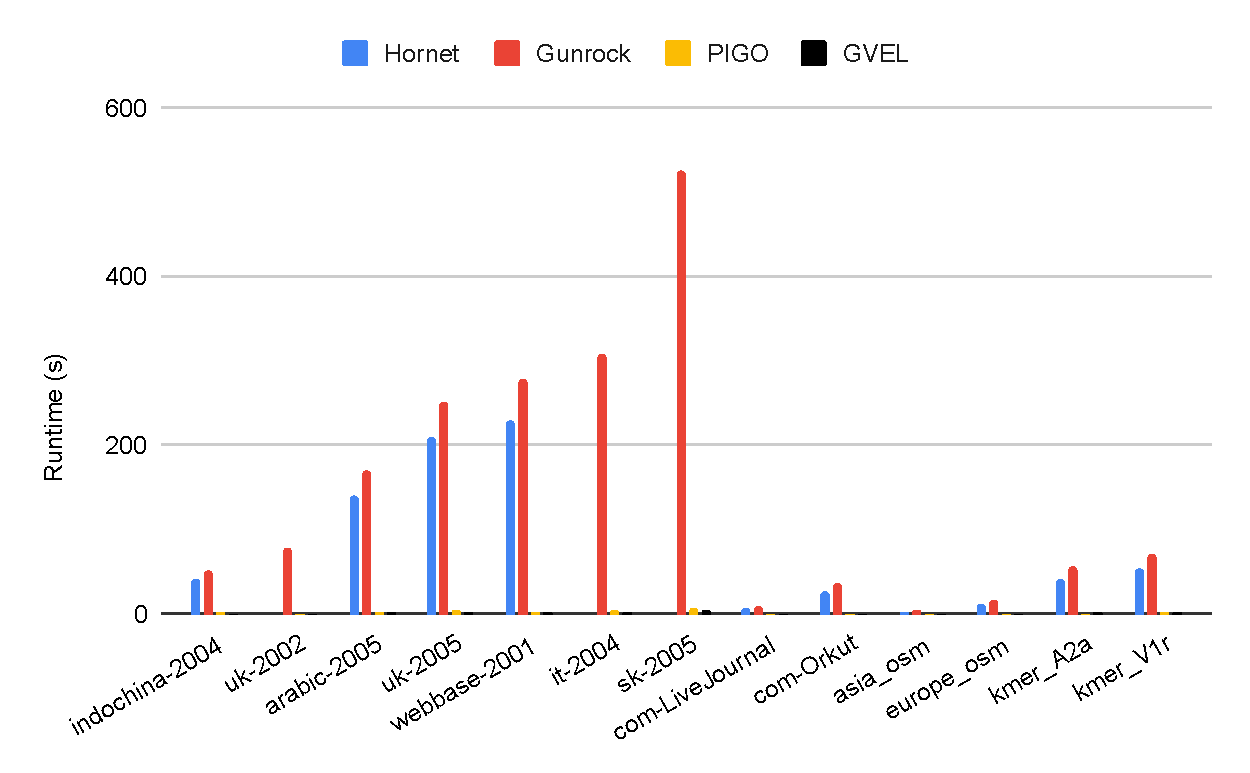
\includegraphics[width=0.68\linewidth]{out/compare-large.pdf} \\[-2ex]
  \caption{Time taken by Hornet, Gunrock, PIGO, and GVEL for reading edge-list and converting it to CSR on 13 different graphs. PIGO and GVEL are not visible on this scale - they are significantly faster than Hornet and Gunrock. The graph loading time for Hornet is not shown for \textit{uk-2002}, \textit{it-2004}, and \textit{sk-2005} graphs as it crashed while loading.}
  \label{fig:compare-large}
\end{figure*}

\begin{figure*}[hbtp]
  \centering
  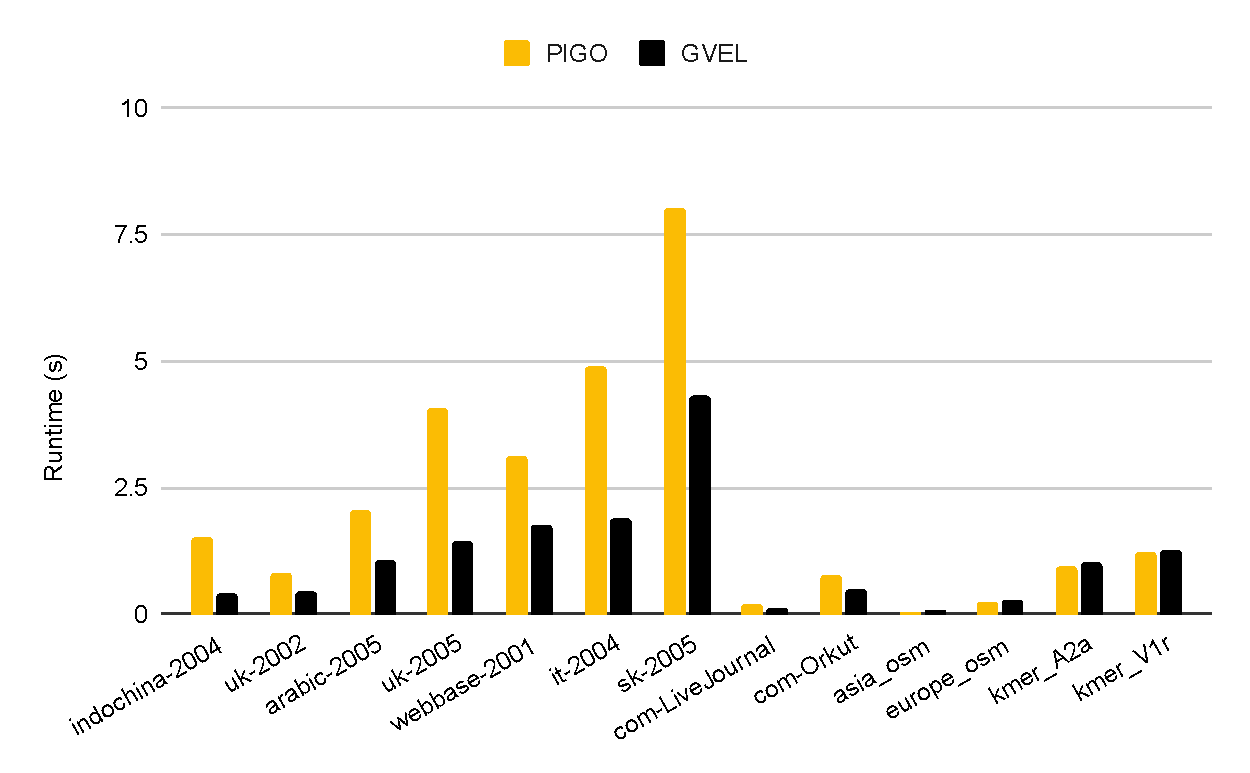
\includegraphics[width=0.68\linewidth]{out/compare-small.pdf} \\[-2ex]
  \caption{Gini coefficient of PageRank values on 24 different graphs, comparing between PageRank values obtained with three different dead-end handling strategies: \textit{teleport from dead-ends} (\textbf{default}), \textit{self-loop dead-ends} (\textbf{loop}), and \textit{self-loop all vertices} (\textbf{loopall}).}
  \label{fig:compare-small}
\end{figure*}


% The efficiency of reading an edgelist stands out, significantly outpacing the speed of reading a graph stored as CSR, which necessitates an additional conversion step. Surprisingly, the average cost of converting an edgelist to CSR is three times higher than simply reading an edgelist from a file. This underscores the notable speed of modern I/O processes. In the sk-2005 dataset, our approach achieves an impressive reading speed of 1.9 billion edges per second. Notably, it's essential to clarify that the table represents edges as directed, not undirected. To visually represent the edge reading performance across different graphs, we propose the inclusion of a plot illustrating this metric. The sluggishness in CSR reading is justified by its nature as a shared data structure, leading to high contention when multiple threads concurrently attempt to add an edge to the same vertex. The process of adding to CSR structures with small degrees is hampered by false sharing, introducing cache coherency issues that contribute to decreased performance.




\subsection{Performance Comparison for Reading Edgelist}

In Figure \ref{fig:compare-el}, we compare the performance of GVEL for reading Edgelist with PIGO. As before, we measure the Edgelist reading time with each framework five times, for averaging. GVEL is on average $2.6\times$ faster than PIGO - with little skew, i.e., GVEL is more or less equivalently faster than PIGO on all graphs. This is more probably than not, due to the reading of Edgelist being \textit{pleasingly parallel}. On the \textit{sk-2005} graph, GVEL achieves a read performance of $1.9$ billion edges/s. Figure \ref{fig:runtime} illustrates the time GVEL requires to read the edge-list and convert it to CSR for each graph in the dataset, presented separately.

\begin{figure*}[hbtp]
  \centering
  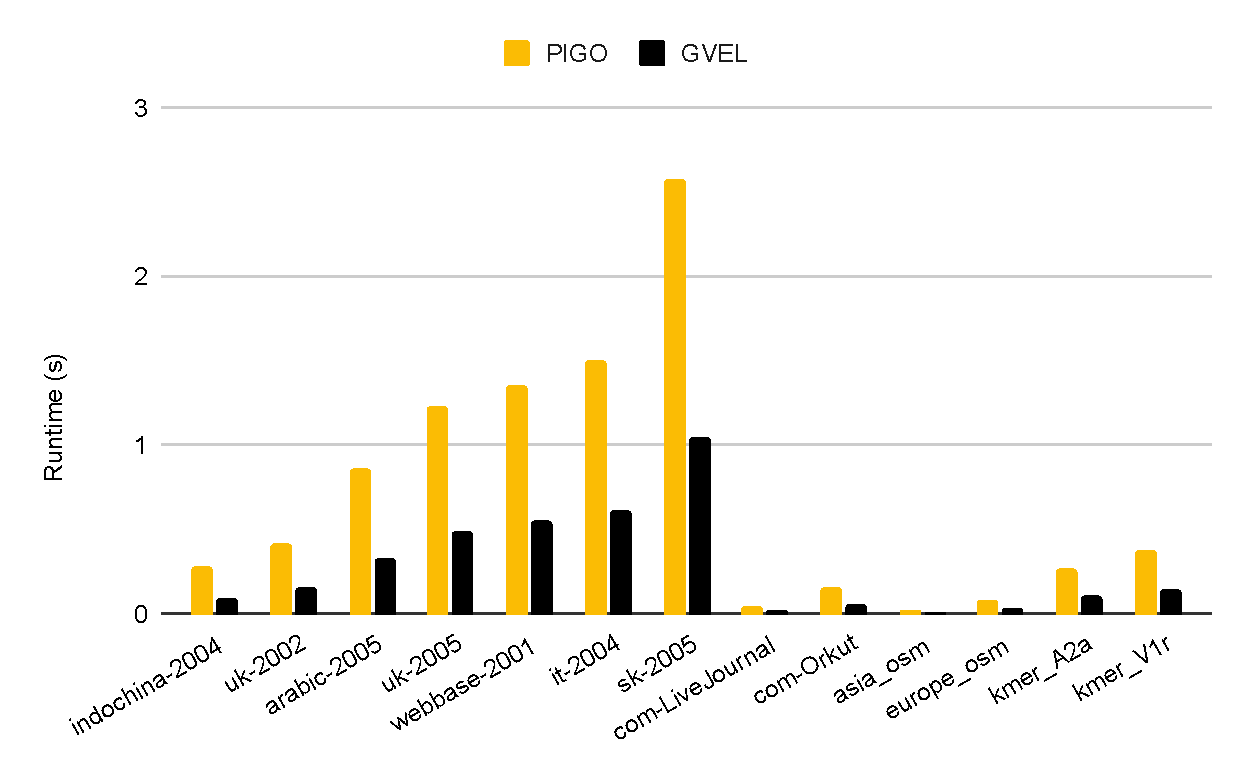
\includegraphics[width=0.68\linewidth]{out/compare-el.pdf} \\[-2ex]
  \caption{Time taken by PIGO and GVEL for reading Edgelist on 13 different graphs.}
  \label{fig:compare-el}
\end{figure*}

\begin{figure*}[hbtp]
  \centering
  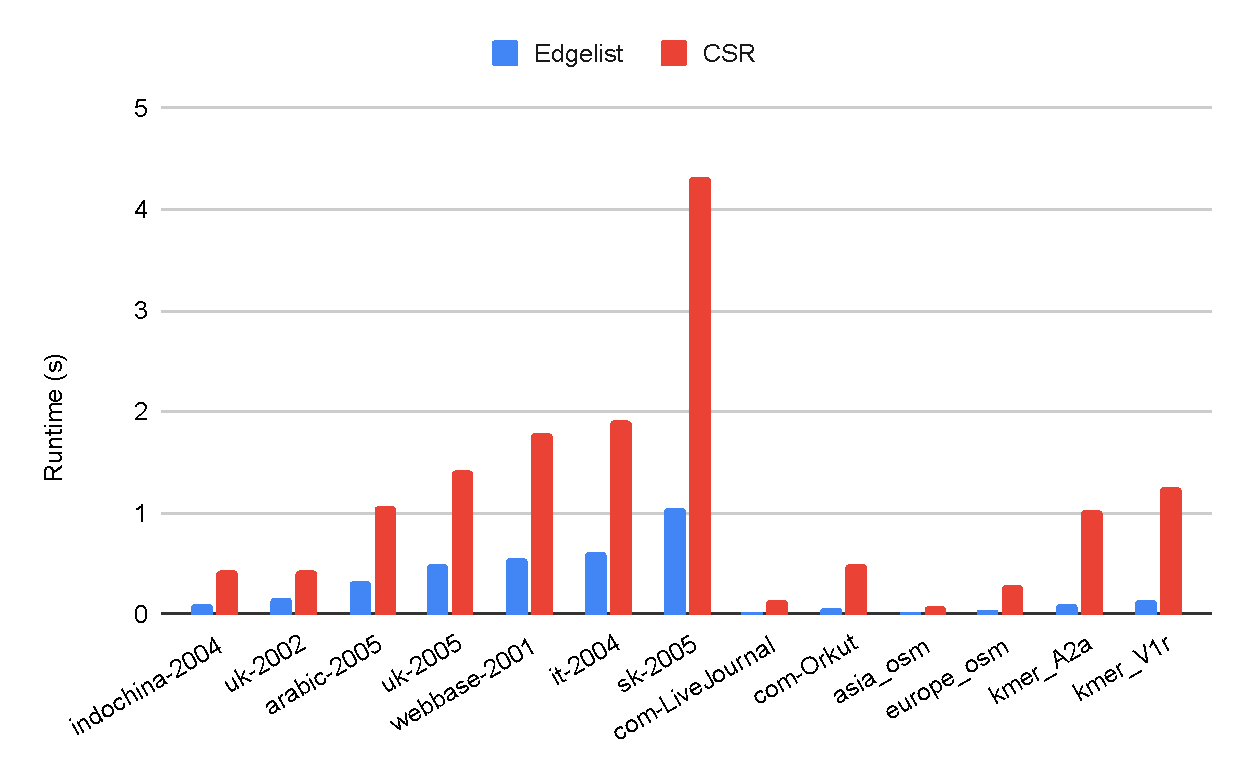
\includegraphics[width=0.68\linewidth]{out/runtime.pdf} \\[-2ex]
  \caption{Time taken by GVEL for edge-list and CSR loading on 13 different graphs.}
  \label{fig:runtime}
\end{figure*}





\subsection{Strong Scaling of GVEL}

Finally, we measure the strong scaling performance of GVEL. To this end, we adjust the number of thread from $1$ to $64$ in multiples of $2$ for each input graph, and measure the time taken for reading Edgelist and reading CSR (reading Edgelist + converting to CSR). As for each experiment above, for each graph, and for each thread count, we perform graph loading five times for averaging. The results are shown in Figure \ref{fig:strong-scaling}. With 32 threads, reading Edgelist with GVEL obtains a $25.0\times$ speedup compared to running with a single thread, i.e., the performance of Edgelist reading increases by $1.9\times$ for every doubling of threads. Further, with 32 threads, reading CSR with GVEL obtains a speedup of $13.9\times$ with respect to a single threaded execution, i.e., the CSR reading performance increases by $1.7\times$ for every doubling of threads. This drop in increase of speedup is due that fact that CSR is a shared data structure, leading to high contention when multiple threads concurrently attempt to add an edge to the same vertex, especially for vertices with high degrees. Further, the process of adding edges to vertices with small degrees is hampered by false sharing of cache lines, which contribute to decreased performance. At 64 threads, both reading Edgelist and reading CSR are impacted by NUMA effects, and offer speedups of only $27.2\times$ and $16.4\times$ respectively.

\begin{figure*}[hbtp]
  \centering
  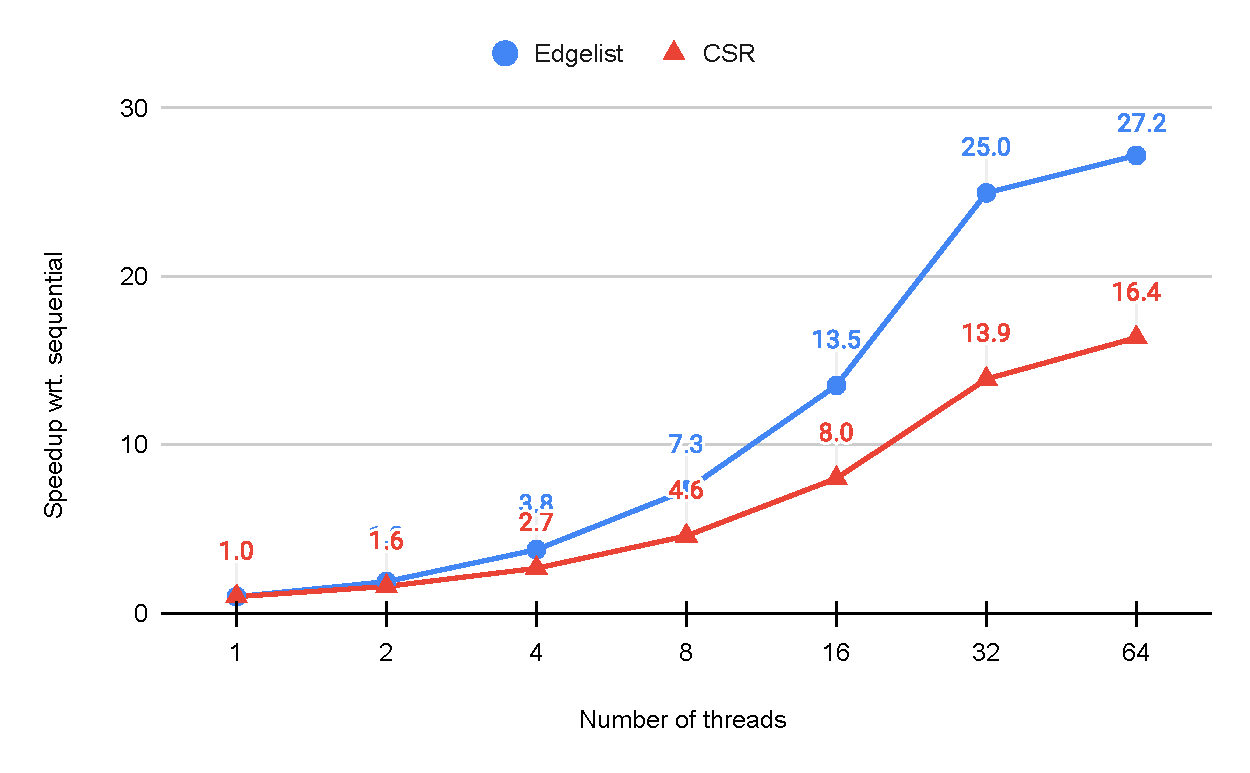
\includegraphics[width=0.68\linewidth]{out/strong-scaling.pdf} \\[-2ex]
  \caption{Speedup of GVEL's Edgelist and CSR loading with increasing number of threads.}
  \label{fig:strong-scaling}
\end{figure*}





% \textbf{Figure 3}:


% We observe that:
% - reading edgelist is significantly faster than reading a graph as CSR (this requires and additional conversion step)
% - in fact, on average, converting an edgelist to CSR is 3 times more costly than reading and edgelist from file (which is quite surprising indded). This shows that modern IO is fastr (dhooom).
% - We are able to read 1.9B edges per second (the table put edges as directed not undirected) in sk-2005.
% - Can we have a plot on edge reading performance per graph
% - (Justify why CSR reading is slow) converting to CSR is slow becuase it is a shared data structure resulting in high contention beteen thread, when multiple threads attempt to add an edge to the same vertex.
% - Also adding to CSR with small degrees suffer from false sharing (cache coherency issue).

% \textbf{Figure 4}:





% Our observations reveal:

% Reading edgelists exhibits impressive scalability, achieving a remarkable 25x scale on 32 threads.
% However, at 64 threads, performance is impacted by NUMA effects.
% Notably, reading CSR does not scale as well, primarily due to issues such as false sharing and contention.
% The influence of NUMA effects is also discernible in CSR reading performance.
% The scaling pattern follows multiples of 2 (linear Y-axis, logarithmic X-axis).

% There is a paper called "Efficient Memory Mapped File I/O for In-Memory File Systems" on the topic - where Choi et al. working at Samsung say that mmap() is a good interface for fast IO (in contrast to file streams) and propose async map-ahead based madvise() for low-latency NVM storage devices. The also have a good slides on this - where their (modified) extended madvice obtains ~2.5x better performance than default mmap() by minimizing the number of page faults.
% I tried parsing integers from text and saving into per-thread integer lists. To over-allocate memory for per-thread integer-lists i use sufficient size mmap() instead of malloc(). Even if i over-allocate, due to virtual memory, only memory as much i need is actually used.


\section{Conclusion}
\label{sec:conclusion}
The study highlights that inequality is prevalent in web graphs, and demonstrates that efforts to minimize it are more effective in contexts with high Gini coefficients. The choice of heuristics plays a crucial role in reducing inequality. Our research suggests that a combination of \textbf{edgeInsertCxrx} and \textbf{edgeInsertCxSx} heuristics may offer an effective approach to minimize inequality. Future research should continue to explore strategies to mitigate inequality in web ranking algorithms and promote a more equitable web environment.


%% The acknowledgments section.
\begin{acks}
I would like to thank Prof. Kishore Kothapalli and Balavarun Pedapudi for their support.
\end{acks}

%% Bibliography style to be used, and the bibliography file.
\bibliographystyle{ACM-Reference-Format}
\bibliography{main}
\end{document}
\endinput
%% End of file.




%% NOTES:
%% - Parallelization seems to be not efficient for small batch updates.
%% - Discuss about conflicting updates
%% - 


%% TODO:
%% - Scale up the size of the graphs
%% - Move experiments to a better server
%% - Include a weak- and strong- scalabiilty plot: run the expt from 2 to 128 threads
%% - overall space planning
%% - add a few lines on novelty of the paper.
%% - table comparison of related work
%% - Include a section on preliminaries that talks about the various algorithmic ideas (Louvain, Label Propagation)

%% Workplan:
%% - KK -- Read Introduction, Related Work,
%% - Dip Sankar -- Approach -- summarize the main algorithmic ideas,
%% - Subhajit -- Results -- Plots, scalability, Dataset, experiments, implementation details,
